Section~\ref{sec:predictionSection} describes the concepts of prediction within the area of wind production and electricity prices. What is important to emphasize here is the type of input data used for the prediction of both price and production. Meteorological factors are important in both cases and can therefore be extracted from the same source. The second type of data is the prices and the productions themselves. Artificial Neural Networks calculates a generalized function by looking at historical data and comparing with the actual values (Section~\ref{sec:annSection}), e.g. comparing the weather factors at time t with the actual production at time t. For this reason it is necessary to collect historical meteorological, price and production data in order to do the prediction. A simple drawing of the input and outout can be seen in Figure~\ref{fig:verySimpleANN}.

\begin{figure}[H]
\centering
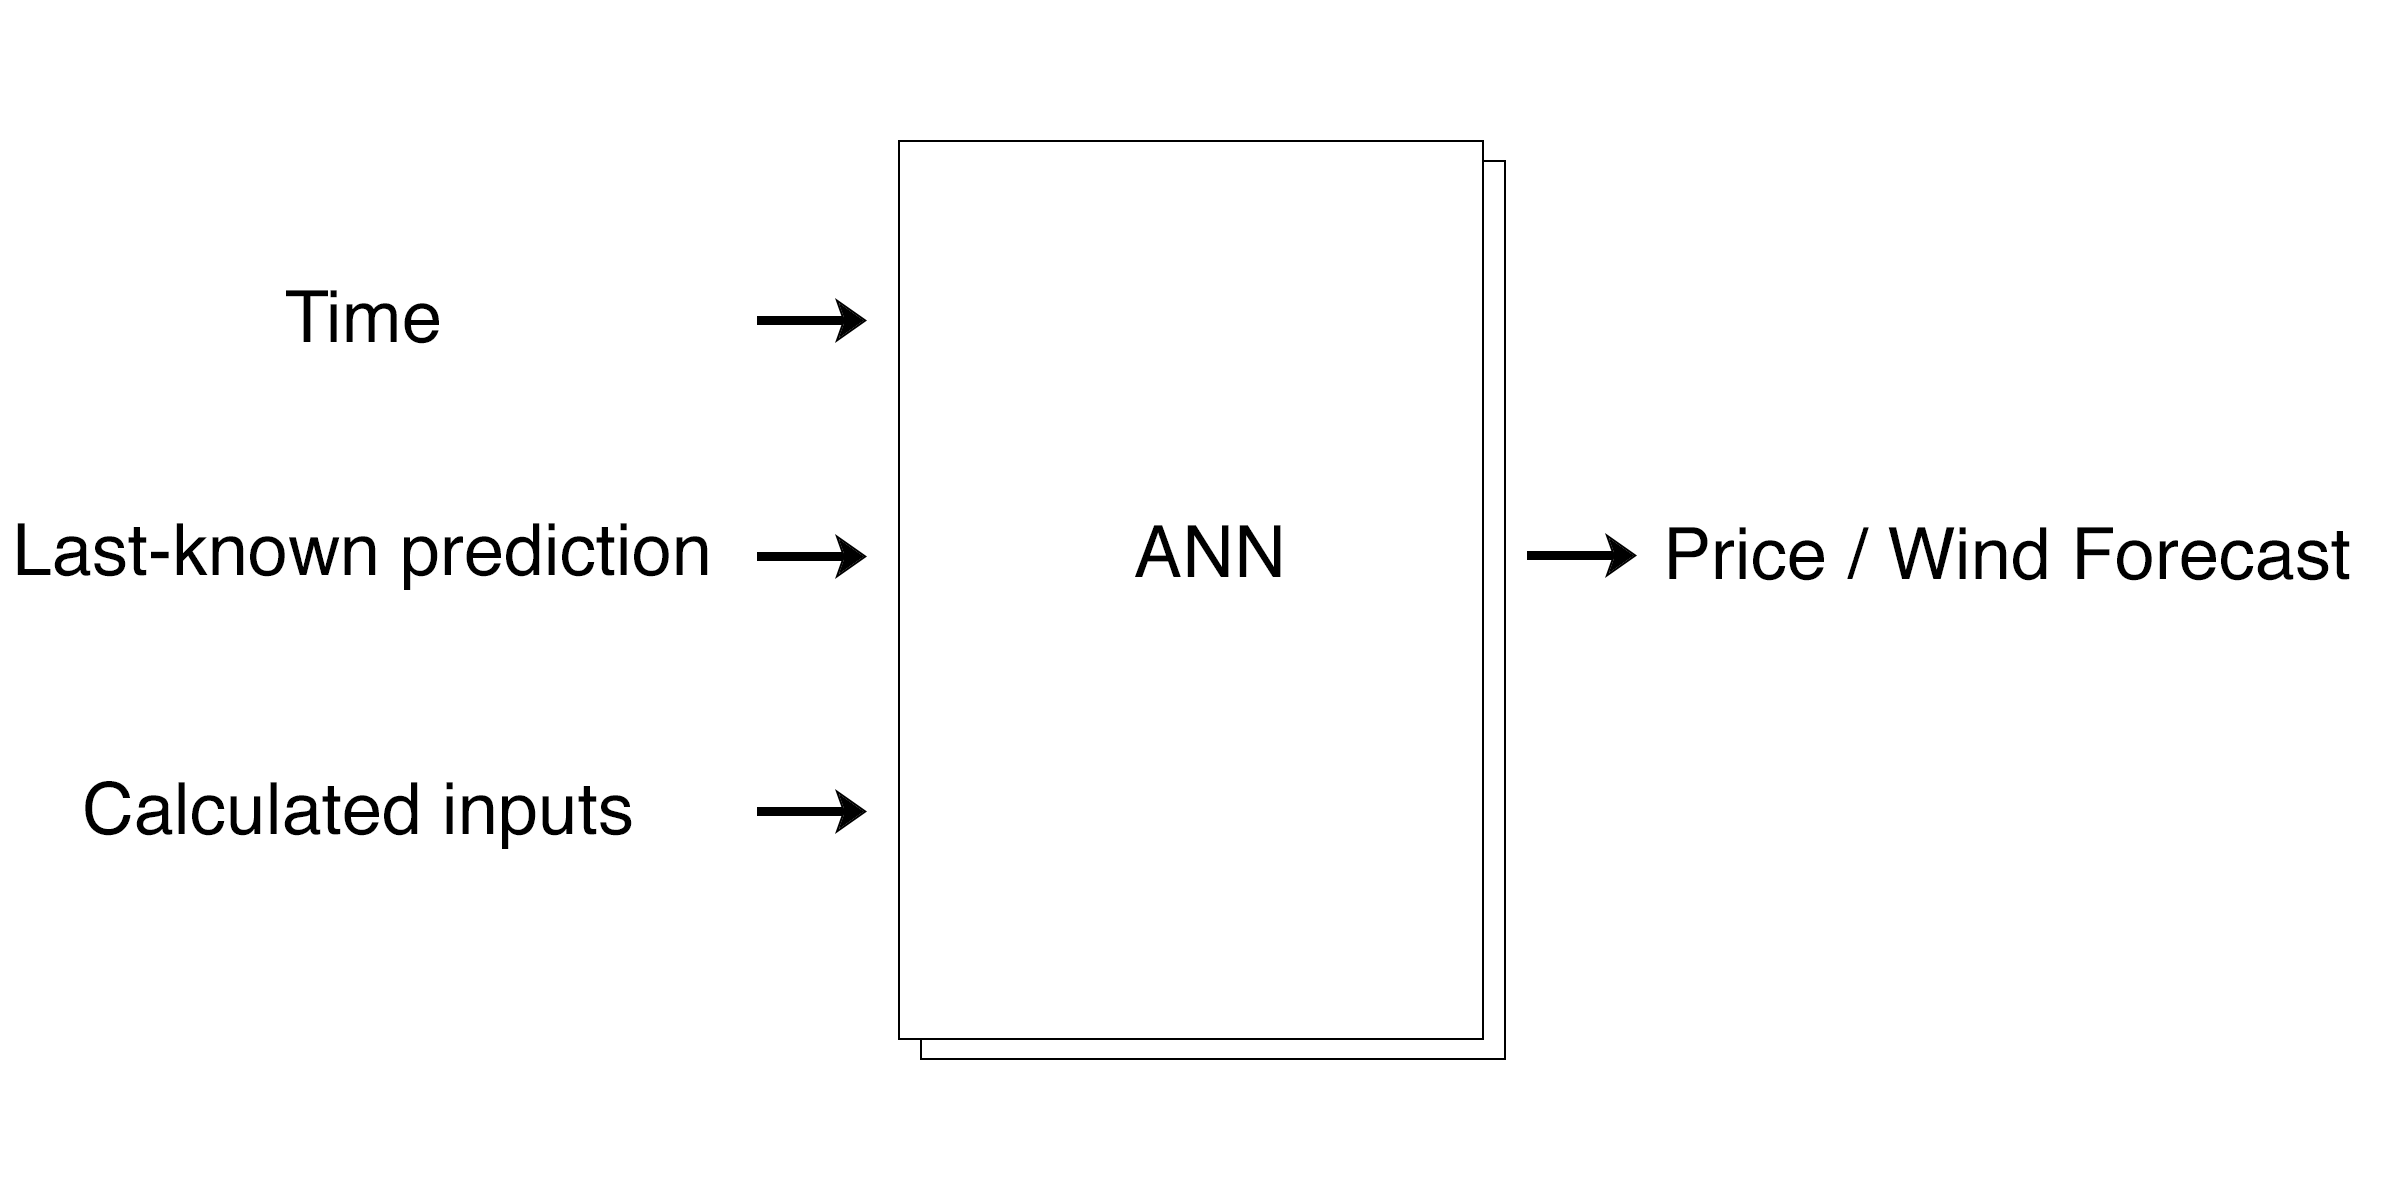
\includegraphics[width=0.85\linewidth,natwidth=898,natheight=587]{billeder/simpleANN.png}
\caption{Simple ANN -- VERY UGLY DRAWING NEED REPLACE}
\label{fig:verySimpleANN}
\end{figure}

The data must come from a trusted source so that proper predictions can be based on it. The data must be of a certain quality in relation number of observations because we need to make hourly predictions, e.g. the meteorological observations must be within an interval of 60 minutes or else we ill ignore data from that particular station.

The National Oceanic and Atmospheric Administration's (NOAA) National Climatic Data Center (NCDC) provides public access to all climate and historical weather data from various weather stations around the world\footnote{\url{http://www.ncdc.noaa.gov/}}. We have used it for collection of historical weather data from various Danish weather stations that delivers observations from at least every hour. The data is in a fixed length format and contains all the necessary weather data for prediction. Format can be seen in \todo{BILAG 11111}. 
The historical hourly price and wind production data has been downloaded from nordpoolspot\footnote{\url{www.nordpoolspot.com}} in excel format BILAG2.
The data will be aggregated into one file that contains the needed input and output parameters for both prediction of price and wind production. The file includes all meteorological factors, prices, consumptions and wind productions from every hour of the last two years. 

For the sake of simplicity we will be focusing on West Denmark and Funen which is also known as DK1 in the electricity market [find ref]. The collected data will be validated through plot diagrams that show and establish the relationships between weather conditions and the power generation/price of DK1.

The weather data is collected from all available weather stations in DK1 from NOAA~\ref{fig:stations4average} - some stations have been omitted due to missing data. The collected data will be averaged and used as basis for creating training sets to be used as input parameters for the Artificial Neural Networks. It is necessary to average the weather data to get a representative picture for all regions included in DK1 because only one price and production exist for all of DK1.

\begin{figure}[H]
\centering
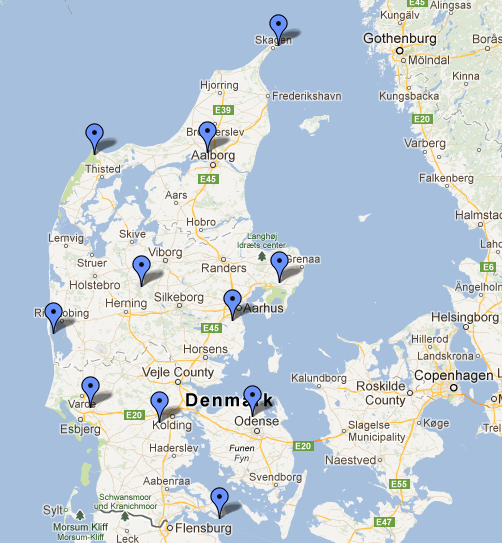
\includegraphics[width=0.85\linewidth,natwidth=898,natheight=587]{billeder/stations4average.png}
\caption{Selected weather stations in DK1}
\label{fig:stations4average}
\end{figure}


We will remove data that is obscure and is related to conditions we cannot predict. (See trimming~\ref{sec:Trimming})